\documentclass[10pt,a4]{article}
\usepackage[english]{babel}
\usepackage[utf8x]{inputenc}
\usepackage{amsmath}
\usepackage{graphicx}
\usepackage[colorinlistoftodos]{todonotes}
\usepackage{hyperref}
\usepackage{geometry}
\geometry{top=3cm,left=2cm,right=2cm,bottom=3cm}
\usepackage[scaled]{helvet}
\usepackage[T1]{fontenc}
\renewcommand\familydefault{\sfdefault}


\author{A. Furlan \and T. F. Costantini}
\date{\today}
\title{An RTEMS device driver for the Bosch BMP180 I2C pressure sensor}



\begin{document}
\maketitle
\tableofcontents

\begin{center}
NOTE: IT IS MANDATORY TO FILL IN ALL THE SECTIONS AND SUBSECTIONS IN THIS TEMPLATE
\end{center}

\section{Project data}

\begin{itemize}
\item 
  Project supervisor(s): Emilio Corigliano

\item 
The group delivering this project:

\begin{center}
\begin{tabular}{lll}
Last and first name & Person code & Email address\\
\hline
  Furlan, Alberto & 10730756 & alberto2.furlan@mail.polimi.it \\
  Costantini, Tommaso Fabrizio & 10918262 & tommasofabrizio.costantini@mail.polimi.it \\
\end{tabular}
\end{center}

\item
How the development tasks were subdivided among the members of the group:

\todo[inline]{TO FILL IN: who did what. The work splits naturally into the
BMP180 driver and its ioctl ABI; the STM32F4 I2C bus driver and its recovery
sequence; the application layer and the lock-free snapshot; the telemetry wire
format and the host-side analysis tooling; and the board bring-up and hardware
validation campaign. Assign these to the two of you as they actually happened.}

\item Public repository hosting the project source code:

\begin{itemize}
\item Repository: \url{https://github.com/AlbertoFurlan20/ES2025}
\item Firmware: \texttt{C\_src/} --- driver, bus, application layer, telemetry.
\item Host analysis tooling and captured datasets: \texttt{E\_analysis/}.
\item Version history and rationale for every change: \texttt{CHANGELOG.md}.
\end{itemize}

\end{itemize}


\section{Project description}

\begin{itemize}
\item \textbf{What is your project about?}
\end{itemize}

The project is a device driver, written from scratch, for the Bosch BMP180
digital barometric pressure and temperature sensor, running under
\textbf{RTEMS 7} on an \textbf{STM32F4-Discovery} board (Cortex-M4,
\texttt{arm/stm32f4} BSP). The sensor is an I2C slave at address \texttt{0x77};
the deliverable is the software stack that turns it into an ordinary RTEMS
device node, \texttt{/dev/bmp180-0}, that any task can \texttt{open()} and
\texttt{ioctl()}.

It took four modules rather than one, because the BSP does not provide
everything the driver needs:

\begin{center}
\begin{tabular}{lll}
Module & Directory & What it is \\
\hline
\texttt{bmp180/} & \texttt{C\_src/src/bmp180/} & the sensor driver --- the scope of the assignment \\
\texttt{i2c/} & \texttt{C\_src/src/i2c/} & a polled STM32F4 I2C master, since the BSP ships none \\
\texttt{bmp\_app/} & \texttt{C\_src/src/bmp\_app/} & application layer: one sampler task owns the device \\
\texttt{telemetry/} & \texttt{C\_src/src/telemetry/} & measurement stream out over USART2, operator commands in \\
\end{tabular}
\end{center}

The stack is complemented by a host-side Python package
(\texttt{E\_analysis/}) that captures the serial stream and computes the noise,
timing and drift statistics used to validate the driver against the datasheet.
No statistics are computed on the target: the board emits raw records and the
numbers are derived on the host, so they can be recomputed without reflashing.

\begin{itemize}
\item \textbf{Why it is important for the AOS course?}
\end{itemize}

The project exercises, on real hardware, most of the topics the course covers
about the boundary between an operating system and the devices it drives:

\begin{itemize}
\item \emph{The driver model.} The driver plugs into the RTEMS generic I2C
  framework (\texttt{libdev/i2c}). A \texttt{bmp180\_dev\_t} has an
  \texttt{i2c\_dev} as its first member so the framework can upcast safely, and
  registration publishes an IMFS node that owns the device, so the node's
  destroy handler frees it rather than the caller. Getting that ownership
  backwards is a use-after-free, which we hit (Section \ref{sec:problems}).
\item \emph{The system-call surface.} The public interface is a frozen ioctl
  ABI (\texttt{\_IOR}/\texttt{\_IOW} encodings, Section
  \ref{sec:design}), which is the concrete form of the userspace/kernel contract
  discussed in the course.
\item \emph{Scheduling and priority.} The final design is three tasks at fixed
  priorities, with every consumer \emph{below} the producer. Getting the
  interaction wrong cost a measured 2.70~s console blackout: a priority-2 task
  busy-looping on a failing ioctl starved every task below it.
\item \emph{Concurrency without blocking the real-time path.} The application
  layer publishes measurements through a seqlock rather than a mutex, so a
  reader can never delay acquisition.
\item \emph{Bounded blocking and fault containment.} Every I2C poll has a 5~ms
  deadline and every conversion wait a datasheet-derived maximum, so a
  disconnected or wedged sensor degrades into an error record instead of a
  system freeze.
\item \emph{Timing as a measurable property.} Because
  \texttt{rtems\_task\_wake\_after(n)} blocks for between $n-1$ and $n$ ticks,
  an unpadded conversion timeout can expire while the sensor is still within
  specification. That one tick of rounding was a stochastic defect in our first
  release, visible only in the noise statistics.
\end{itemize}

This is not an open source project contribution, so there is no upstream
maintainer correspondence to report.

\subsection{Design and implementation}
\label{sec:design}

The full source is in the repository under \texttt{C\_src/}; what follows is the
structure.

\paragraph{Layering.} One folder per module, mirrored across \texttt{src/},
\texttt{inc/} and \texttt{tests/}. Only \texttt{inc/} is on the include path,
never \texttt{inc/<module>/}, so every include names the module it reaches into
(\texttt{\#include "bmp\_app/app.h"}). Dependencies only ever point downwards:
\texttt{bmp180/} knows nothing of \texttt{bmp\_app/}, and \texttt{bmp\_app/}
knows nothing of \texttt{telemetry/}. \texttt{init.cpp} and
\texttt{constants.h} sit at the top because they belong to the image rather
than to any module.

\paragraph{The bus driver (\texttt{i2c/}).} The \texttt{arm/stm32f4} BSP ships
no driver for the modern \texttt{<dev/i2c/i2c.h>} framework, so the sensor
driver had nothing to sit on. We wrote a polled master bus driver that
registers as \texttt{/dev/i2c-1}: peripheral clock gating, GPIO alternate
function mux, CCR/TRISE clock math against \texttt{PCLK1} (16~MHz on this BSP)
for 100~kHz standard mode, and start/address/data/stop sequencing. Every status
poll is bounded by \texttt{I2C\_POLL\_TIMEOUT\_US = 5000}. Everything that
differs between I2C1, I2C2 and I2C3 is isolated in a \texttt{stm32f4\_i2c\_hw}
descriptor; the transfer engine is instance-agnostic.

It also carries a \emph{bus recovery} sequence. A CPU reset landing mid-transfer
leaves the BMP180 holding SDA low waiting for clock pulses that never arrive;
the peripheral latches BUSY and every transfer returns \texttt{-EBUSY}. Before
this was added, only a power cycle cleared it. Recovery takes the pins away from
the peripheral, drives up to nine SCL pulses by hand (eight data bits plus the
ACK), issues a manual STOP, software-resets the peripheral and restores the
configured clock. A line shorted to ground cannot be freed this way
and is reported as a distinct error.

\paragraph{The sensor driver (\texttt{bmp180/}).} \texttt{bmp180\_register()}
allocates the device through the framework, reads the chip ID register
(\texttt{0xD0}, expecting \texttt{0x55}) and publishes the node. A registration that succeeds proves the wiring,
not the calibration. The eleven 16-bit calibration coefficients are read once,
lazily, on the first measurement and cached in the device context.
\texttt{bmp180\_unregister()} goes through \texttt{unlink()}, since the IMFS node
owns the device.

The public interface exposed on the node is:

\begin{verbatim}
  ioctl(fd, BMP180_IOCTL_READ_MEASUREMENT,  &result) // bmp180_measurement_t
  ioctl(fd, BMP180_IOCTL_SET_OSS,           &oss)    // bmp180_oss_t
  ioctl(fd, BMP180_IOCTL_GET_OSS,           &oss)    // bmp180_oss_t
  ioctl(fd, BMP180_IOCTL_SOFT_RESET)                 // no payload
  ioctl(fd, BMP180_IOCTL_SET_TEMP_INTERVAL, &ms)     // uint32_t
  ioctl(fd, BMP180_IOCTL_GET_TEMP_INTERVAL, &ms)     // uint32_t
\end{verbatim}

A measurement is returned as a \texttt{bmp180\_measurement\_t}: temperature in
steps of $0.1\,^{\circ}$C and pressure in Pa. The Bosch compensation algorithm
is implemented verbatim from datasheet section 3.5 (Figure 4) in
\texttt{int32\_t}/\texttt{int64\_t} arithmetic, so the image carries no
floating-point dependency in the measurement path.

Two design decisions inside the driver:

\begin{itemize}
\item \emph{Conversion waits are polled, not slept through.} The driver sleeps
  the datasheet \emph{typical} conversion time, then polls the SCO bit of
  \texttt{ctrl\_meas} until the sensor reports the conversion finished, giving
  up at the datasheet \emph{maximum} plus one tick of padding. Reaching the
  maximum is an error (\texttt{ETIMEDOUT}), not a slow sample.
\item \emph{Temperature is cached.} Pressure compensation needs a temperature,
  not a \emph{fresh} temperature, and the datasheet notes temperature can be
  measured far less often than pressure. Re-reading it every cycle spent a whole
  extra 3--6~ms conversion on a quantity that moves in minutes. The interval is
  1000~ms by default and settable per device; 0 restores one temperature
  conversion per measurement.
\end{itemize}

\paragraph{The application layer (\texttt{bmp\_app/}).}
\texttt{bmp\_app\_sampler\_task} is the only task that opens
\texttt{/dev/bmp180-0}: it acquires back-to-back and publishes each measurement
into a one-deep snapshot. Consumers call \texttt{bmp\_app\_read()}, which never
blocks and adds no bus traffic, and change the mode or the temperature interval
through setters the sampler applies at the top of its next cycle. \texttt{oss}
therefore has exactly one writer, and no consumer holds a descriptor on the
device.

The snapshot is a \textbf{seqlock}, not a mutex: the sequence counter is odd
while a publish is in progress and even when the payload is stable, and readers
retry. An RTEMS mutex held by a low-priority reader would block the sampler
until the priority-inheritance handoff completed; here the reader simply retries
and the writer never waits at all.

\emph{A successful read does not mean a fresh reading.} A failed cycle does not
publish, so a sensor that stops answering leaves the last good sample, with its
last good timestamp, in place indefinitely. Consumers detect it by comparing \texttt{seq} against their previous read, or
\texttt{t\_us} against the current uptime, and learn the reason from
\texttt{bmp\_app\_last\_error()}.

\paragraph{The telemetry layer (\texttt{telemetry/}).}
\texttt{bmp180\_telemetry\_task} is a consumer like any other: it holds no
descriptor and issues no ioctl. It subscribes to the sampler
(\texttt{BMP\_APP\_EVENT\_SAMPLE}), drives the validation profile through
\texttt{bmp\_app\_set\_oss()}, and writes records to USART2. The wire format is frozen at v1 and machine-readable:

\begin{center}
\begin{tabular}{ll}
Record & Meaning \\
\hline
\texttt{\#BMP180 v1 fw=... temp\_ms=...} & session header, written once before any record \\
\texttt{S <t\_us> <t\_cdeg> <p\_pa> <oss>} & one sample \\
\texttt{E <t\_us> <errno>} & an acquisition error, reported on the edge \\
\texttt{D <t\_us> <lost>} & samples the consumer missed \\
\end{tabular}
\end{center}

The timestamp in an \texttt{S} record is the one the \emph{sampler} took at
acquisition, never the time the telemetry task happened to run, because the host
derives the achieved rate and the jitter from differences between consecutive
records. Errors are emitted on the edge: a disconnected sensor fails hundreds of
times a second and would otherwise flood the console.

\paragraph{The control surface (\texttt{telemetry/control.cpp}).} The same
USART2 that carries telemetry out carries operator commands in, on \texttt{PA3}.
\texttt{bmp180\_control\_task} owns the read side and is the only task that reads
\texttt{stdin}. Like the telemetry task it is a consumer of \texttt{bmp\_app}: a
command becomes a \texttt{bmp\_app\_set\_oss()} or a
\texttt{bmp\_app\_request\_soft\_reset()}, applied by the sampler at the top of
its next cycle. One command per line:

\begin{center}
\begin{tabular}{ll}
Line & Effect \\
\hline
\texttt{O0}--\texttt{O3} & switch to that oversampling mode \\
\texttt{R} & soft reset; the device returns to power-on defaults \\
\end{tabular}
\end{center}

Anything else is discarded. The task never writes to the console, since an echo
or an error message would appear in every capture as a line the host parser has
to skip; the console is put into canonical mode with echo off at startup for the
same reason. Confirmation comes from the \texttt{oss} field of the next samples,
which reports the mode they were taken at.

The first accepted command cancels the boot sweep (\texttt{telem\_cancel\_sweep}):
the sweep steers \texttt{oss} itself and keys each block on getting the mode it
asked for, a condition that can never match again once an operator sets the mode.
A capture used for validation is one where no command was typed.

\paragraph{Tasks and priorities.} The image runs three tasks after
initialisation:

\begin{center}
\begin{tabular}{lll}
Task & Priority & Role \\
\hline
\texttt{SAMP} & 2 & owns the fd, acquires, publishes, sends the sample event \\
\texttt{TELE} & 3 & reads the surface, drives the sweep, writes USART2 \\
\texttt{CTRL} & 4 & blocks in \texttt{read()} on the console, applies commands \\
\end{tabular}
\end{center}

\texttt{TELE} sits \emph{below} \texttt{SAMP} on purpose. A higher-priority
reader can preempt a publish in progress and burn its retry budget for nothing;
a lower-priority one is guaranteed a stable payload, and still gets the CPU
because the sampler sleeps inside every conversion wait. Symmetrically, the
sampler yields a tick after a \emph{failed} cycle --- without that, a
disconnected sensor turns it into a busy-loop at priority 2 and nothing below it
runs to report the fault.

\texttt{CTRL} sits below both: it is blocked in \texttt{read()} almost always,
and an arriving command must not preempt a publish that \texttt{TELE} is reading.
A console returning EOF or an error would spin the loop, so that case sleeps
100~ms.

\todo[inline]{Before submission: \texttt{C\_src/src/init.cpp} currently creates
\texttt{CTRL} at priority \textbf{2}, tied with \texttt{SAMP}, which contradicts
its own comment (``Control is lowest''), \texttt{control.h} (``run this task
below the telemetry task'') and \texttt{control.cpp} (``spin this loop at
priority 4''). The table above states the intended value, 4. Fix the argument in
\texttt{setupTask(\&control\_task\_id, "CTRL", 2, ...)} or change the table. The
validation captures are unaffected either way: no command was typed during them,
so \texttt{CTRL} stayed blocked in \texttt{read()} and never became runnable.}

\paragraph{Hardware setup.} The examiner needs three connections: the sensor on
I2C1, the USB-serial adapter on USART2, and the ST-Link (the board's own on-board
USB) for flashing.

\begin{center}
\begin{tabular}{lll}
Signal & STM32F4-Discovery pin & Peer \\
\hline
SCL & PB6 & BMP180 SCL \\
SDA & PB7 & BMP180 SDA \\
VDD (3.3~V) & 3V & BMP180 VIN \\
GND & GND & BMP180 GND \\
Console TX & PA2 & CP2102 RXD \\
Console RX & PA3 & CP2102 TXD \\
GND & GND & CP2102 GND \\
\end{tabular}
\end{center}

I2C1 runs at 100~kHz standard mode, sensor address \texttt{0x77}. The console is
USART2, 115200~8N1.

\paragraph{Toolchain and BSP configuration.} Full step-by-step instructions are
in \texttt{B\_docs/SETUP.md}; the short version is: build the
\texttt{7/rtems-arm} toolchain with the RTEMS Source Builder, then configure and
install the \texttt{arm/stm32f4} BSP with \texttt{waf}.

\textbf{One BSP option is not optional for this project.} The stock
\texttt{arm/stm32f4} BSP puts the console on USART3; we use USART2, so the BSP
must be built with the following \texttt{config.ini} before
\texttt{./waf configure}:

\begin{verbatim}
[arm/stm32f4]
BUILD_TESTS = True
STM32F4_ENABLE_USART_2 = True
STM32F4_ENABLE_USART_3 = False
\end{verbatim}

The resulting setting can be confirmed in the installed
\texttt{.../arm-rtems7/stm32f4/lib/include/bspopts.h}, which should show
\texttt{STM32F4\_ENABLE\_USART\_2} defined and \texttt{STM32F4\_USART\_BAUD
115200}.

\paragraph{Building and flashing.} The toolchain path is written in exactly one
place, \texttt{.env/setup.env}, a single \texttt{KEY=VALUE} line copied from the
committed example. \texttt{compile.sh}, \texttt{flash.sh}, \texttt{Makefile} and
the root \texttt{CMakeLists.txt} all read that file, so the four build paths
cannot drift.

\begin{verbatim}
cp .env/setup.env.example .env/setup.env
# edit it: RTEMS_LOCAL_PATH=/path/to/where/RTEMS_toolchain/lives

cd C_src
./compile.sh        # or: make        -- builds the .exe
make flash          # build + program the board over OpenOCD
\end{verbatim}

Everything is compiled with \texttt{-std=c++17 -Wall -Wextra -Werror
-fno-exceptions -fno-rtti} for Cortex-M4 with hard-float
(\texttt{-mfpu=fpv4-sp-d16}). Flashing goes through OpenOCD with
\texttt{board/stm32f4discovery.cfg}, programming the raw binary at
\texttt{0x08000000}.

\paragraph{Running it.} Attach a serial terminal to the USB-serial adapter and
reset the board (black B2 button, or let \texttt{capture.sh} reset it over the
ST-Link):

\begin{verbatim}
screen /dev/cu.usbserial-0001 115200     # macOS: cu.*, never tty.*
                                         # exit screen: Ctrl-A then \
\end{verbatim}

A healthy boot looks like this:

\begin{verbatim}
[SELFTEST] compensate: T=150 (exp 150)  P=69964 (exp 69964)  -> PASS
#BMP180 v1 fw=2.0.0 temp_ms=1000
[[DEBUG]] BMP180 registered on /dev/bmp180-0
S 1043221 244 96822 0
S 1054220 244 96825 0
\end{verbatim}

The first line is a hardware-independent self-test of the Bosch compensation
math, run at every boot against the datasheet worked example; a \texttt{FAIL}
there means the arithmetic is broken, independently of any wiring problem. The
firmware then registers the bus and the sensor and starts streaming.

\paragraph{Using the driver from your own task.} Two ways, depending on whether
you want to own the device:

\begin{verbatim}
/* Through the application layer -- the normal path. Non-blocking,
   no bus traffic, no descriptor. */
bmp_app_sample_t s;
if (bmp_app_read(&s)) { /* s.pressure_pa, s.temperature_cdeg, s.oss, s.seq */ }
bmp_app_set_oss(BMP180_OSS_ULTRA_HIGH_RES);   /* applied next cycle */
bmp_app_request_soft_reset();                 /* power-on defaults */

/* Directly on the device node -- only if nothing else owns it. */
int fd = open("/dev/bmp180-0", O_RDWR);
bmp180_measurement_t m;
ioctl(fd, BMP180_IOCTL_READ_MEASUREMENT, &m);
\end{verbatim}

\section{Project outcomes}

\subsection{Concrete outcomes}

\paragraph{The firmware.} Repository
\url{https://github.com/AlbertoFurlan20/ES2025}, 58 commits and nine firmware
releases from 1.0.0 to \textbf{2.0.0} (tags \texttt{v1.0.0} through
\texttt{v2.0.0}; 1.6.0 is recorded in the CHANGELOG but was never tagged).
\texttt{CHANGELOG.md} records every release, what changed in the measurement
path and what was measured to justify it, including the defects listed in
Section \ref{sec:problems}.

\begin{center}
\begin{tabular}{lll}
Artifact & Path & Size \\
\hline
BMP180 driver & \texttt{C\_src/src/bmp180/driver.cpp} & 745 lines \\
STM32F4 I2C master & \texttt{C\_src/src/i2c/i2c.cpp} & 622 lines \\
Application layer & \texttt{C\_src/src/bmp\_app/app.cpp} & 229 lines \\
Telemetry and control & \texttt{C\_src/src/telemetry/} & 411 lines \\
Boot and RTEMS config & \texttt{C\_src/src/init.cpp} & 144 lines \\
Public headers & \texttt{C\_src/inc/} & 12 headers \\
\end{tabular}
\end{center}

\paragraph{Host-side tooling and data.} \texttt{E\_analysis/} is a small Python
package split so that the metrics are testable without hardware or a display:
\texttt{parse.py} (stream to DataFrames), \texttt{metrics.py} (DataFrames to
numbers), \texttt{plot.py} (numbers to charts), plus \texttt{capture.sh}, which
resets the target over the ST-Link and writes a timestamped log, plus
\texttt{make\_report\_figures.py}, which renders the figure set used in this
report. The repository carries 44 captures taken during development, including the ones
that record failures, so every sweep, timing and recovery number quoted here can
be recomputed from committed data without a board.

\paragraph{Tests.} Two host-compiled suites that need no toolchain and no
board (\texttt{make -C C\_src/tests run}): the telemetry formatter, and the
seqlock snapshot including a concurrent writer. On the target, the compensation
self-test runs at every boot, and three build flags select fault and teardown
tests that must not be present in a normal build:

\begin{verbatim}
  -DBMP180_TEARDOWN_TEST   -DI2C_RECOVERY_TEST   -DBMP180_NO_BUS_LOCK
\end{verbatim}

\paragraph{Validation.}
\label{sec:testing}
\texttt{C\_src/TESTING.md} is a ten-step validation ladder, from
hardware-independent math up to physical and fault tests, and each step states
what to expect and what a failure means. The quantitative core is an
oversampling sweep: 500 samples in each of the four modes after three discarded
warm-up samples, then a continuous run at \texttt{OSS=2}. No statistics are
computed on the device.

Release 2.0.0 was validated on hardware with \textbf{three consecutive 150~s
captures}, committed as
\texttt{E\_analysis/captures/20260902-165752.log},
\texttt{-170059.log} and \texttt{-170351.log}. Each carries about 13\,640
samples, and all three report \textbf{zero errors, zero dropped records and zero
malformed lines}. Zero drops is what shows that emission never throttled
acquisition, the premise every timing figure rests on.

The acceptance gate for the release was that the four median acquisition
intervals be unchanged from the previous one, since the restructuring touched
who may talk to the device and not the acquisition path. They were identical in
all three runs and identical to the figures recorded for 1.5.0:

\begin{center}
\begin{tabular}{lllll}
\texttt{oss} & $n$ per sweep block & median interval ($\mu$s) & mean pressure, run 1 (Pa) & datasheet RMS (Pa) \\
\hline
0 & 500 & 5000 & 100545.9 & 6.0 \\
1 & 500 & 7000 & 100545.9 & 5.0 \\
2 & 500 & 10999 & 100543.5 & 4.0 \\
3 & 500 & 18999 & 100542.3 & 3.0 \\
\end{tabular}
\end{center}

The interval column is the same in all three runs; the mean-pressure column is
run 1 alone, since absolute pressure moves between runs with the weather. Within
a run, mean pressure is constant across the four modes to within 4~Pa in run 1
and 7~Pa in the worst of the three, as it must be: the true pressure does not
depend on how the sensor is sampled.

\paragraph{The measured history.} Every release was captured the same way, so
the whole development history can be read off the committed data. Twenty-two
captures recorded a complete sweep across eight firmware versions; the remaining
committed captures are deliberate failures (wedged buses, resets landing
mid-transfer) and are excluded, since a partial sweep is not comparable. One of
the two 1.5.0 points is the forced bus-recovery build of Section
\ref{sec:problems} rather than the release binary; it is kept because its four
intervals are identical to the release's, the check that build exists to pass.

\begin{center}
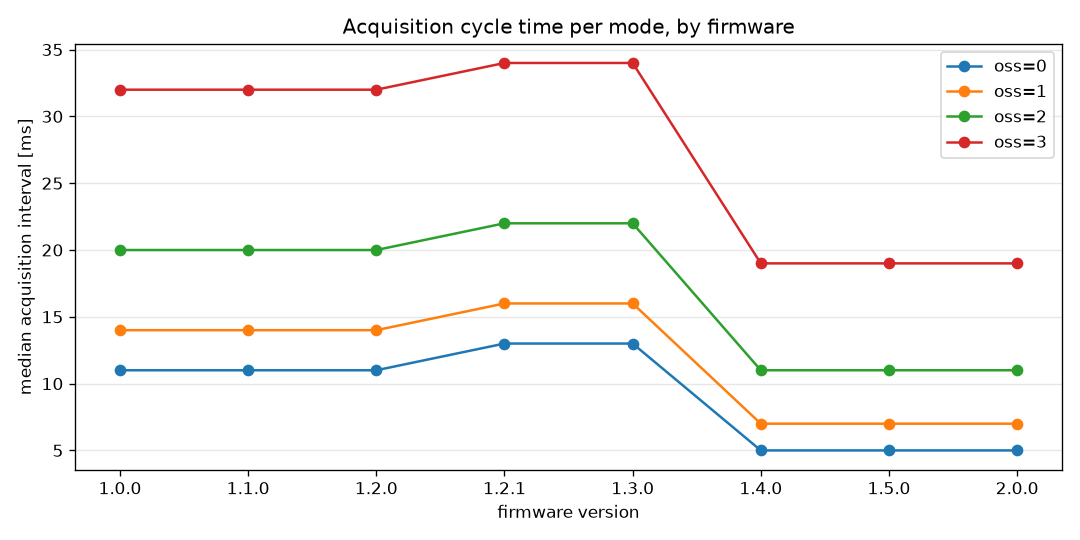
\includegraphics[width=\textwidth]{../E_analysis/figures/v2.0.0/interval_history.png}
\end{center}

Acquisition cycle time has three regimes, and each step is a decision recorded
in \texttt{CHANGELOG.md}:

\begin{itemize}
\item \textbf{1.0.0 to 1.2.0 --- 11 / 14 / 20 / 32~ms.} The driver slept the
  datasheet maximum for the mode and then read the result registers.
\item \textbf{1.2.1 to 1.3.0 --- 13 / 16 / 22 / 34~ms.} Two milliseconds
  \emph{slower} per sample, deliberately. Every conversion constant gained one
  tick of padding, because \texttt{rtems\_task\_wake\_after(n)} blocks for
  between $n-1$ and $n$ ticks and the unpadded waits were occasionally expiring
  while the sensor was still converting: throughput paid for correctness.
\item \textbf{1.4.0 onwards --- 5 / 7 / 11 / 19~ms.} Between 1.7 and 2.6 times
  faster depending on the mode, from two changes at once whose contributions
  separate cleanly. The temperature cache removes one whole conversion, which is
  the same 6~ms whatever the mode, so it dominates the \emph{ratio} at
  \texttt{oss=0} where the cycle was shortest to begin with. SCO polling saves
  the gap between a conversion's padded maximum and its typical time, which
  grows with the mode (3~ms at \texttt{oss=0} against 10~ms at \texttt{oss=3}),
  so it dominates the \emph{absolute} saving at the top mode, where 15 of the
  34~ms disappear. Polling the SCO bit replaced the fixed worst-case sleep, so a
  cycle ends when the conversion ends rather than at its datasheet maximum, and
  most cycles skip the temperature conversion entirely. The padded maxima became
  the timeout rather than the wait.
\end{itemize}

Release 2.0.0 lands on the 1.4.0 line: moving every consumer off the device and
behind an application layer cost the acquisition path nothing.

\begin{center}
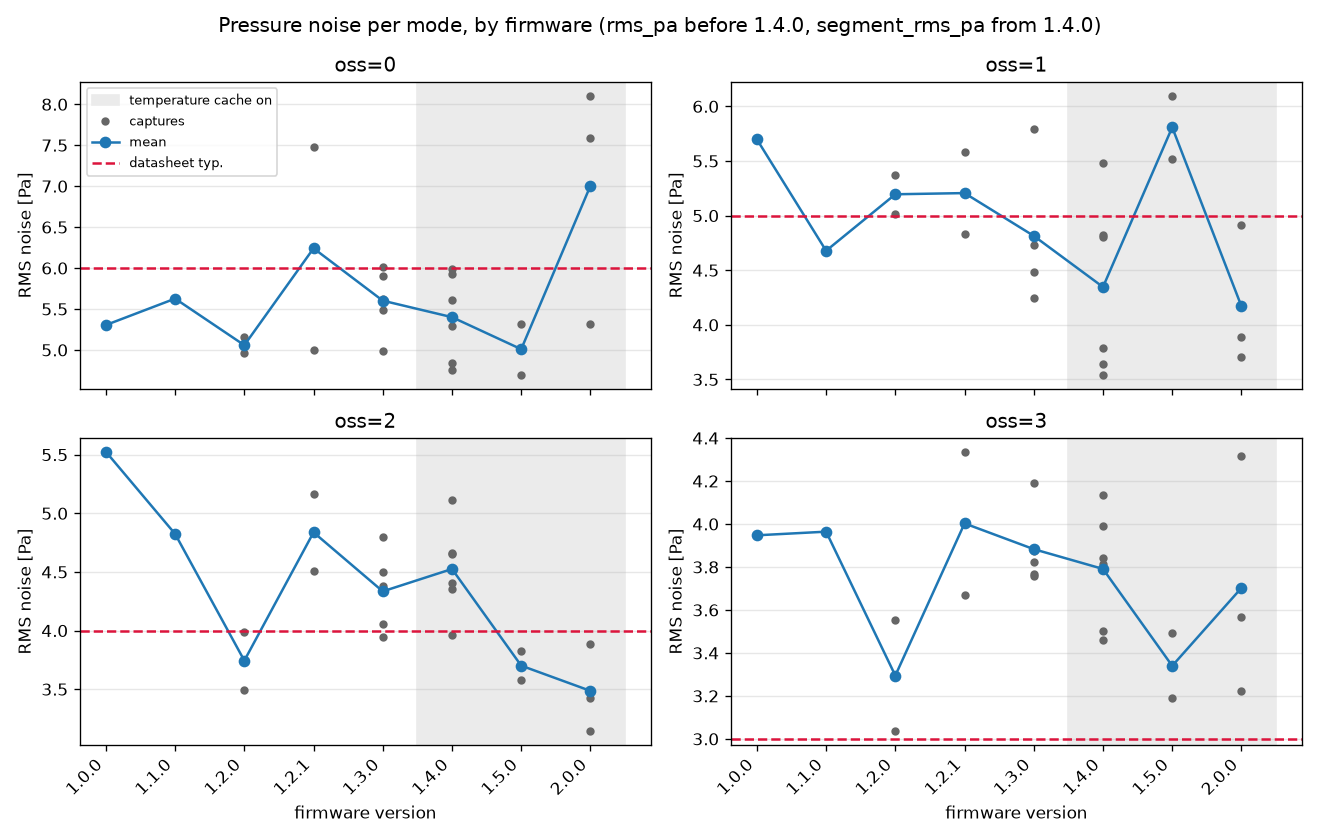
\includegraphics[width=\textwidth]{../E_analysis/figures/v2.0.0/noise_history.png}
\end{center}

Noise shows no such steps. Across all eight versions each mode's per-version
mean stays inside a band at most about 2~Pa wide, near its datasheet figure,
with no trend: the firmware changes moved timing, structure and fault behaviour,
none of which make the sensor quieter or noisier. The two eras are measured with
different columns, whole-block RMS before the temperature cache existed and
median within-segment RMS after it, and the chart marks the boundary rather than
blending them: with the cache off the segments are two or three samples long and
their spread understates the noise. The one visible outlier, \texttt{oss=0} at
2.0.0, is the post-boot settling transient identified below.

Pressure noise is reported per mode as the median within-segment RMS, not the
whole-block RMS. The driver compensates every reading in an interval against one
cached temperature, and compensation moves about 25~Pa per $0.1\,^{\circ}$C, so
a drifting temperature leaves the stream as a staircase and whole-block RMS
would measure thermal drift times the cache interval rather than the sensor.
Across the three runs:

\begin{center}
\begin{tabular}{lllll}
\texttt{oss} & run 1 (Pa) & run 2 (Pa) & run 3 (Pa) & datasheet typ. (Pa) \\
\hline
0 & 5.32 & 7.59 & 8.11 & 6.0 \\
1 & 4.91 & 3.71 & 3.89 & 5.0 \\
2 & 3.89 & 3.43 & 3.14 & 4.0 \\
3 & 3.22 & 4.32 & 3.57 & 3.0 \\
\end{tabular}
\end{center}

\begin{center}
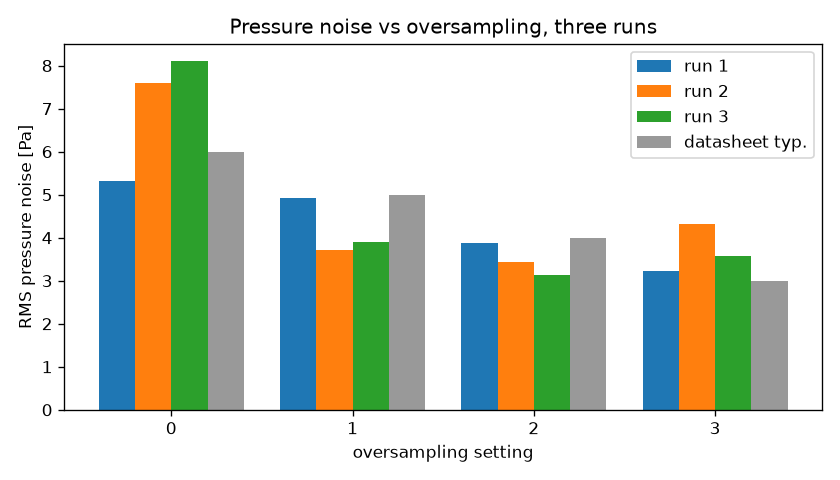
\includegraphics[width=0.78\textwidth]{../E_analysis/figures/v2.0.0/noise_across_runs.png}
\end{center}

Oversampling works: noise falls by roughly a factor of two from \texttt{oss=0}
to \texttt{oss=2} in every run. We do not claim the monotonicity criterion as
passed, though. It holds across the first three modes in all three runs; at the
\texttt{oss=2} to \texttt{oss=3} step it holds in one run of three.

The obvious explanation does not survive. Since the sweep visits each mode once
in sequence, a block's exposure to atmospheric movement grows with the mode
(2.5~s of wall clock at \texttt{oss=0} against 9.5~s at \texttt{oss=3}), so we
fitted and removed a linear pressure trend from each block. At \texttt{oss=3} detrending changes almost nothing (3.22, 4.32
and 3.57~Pa become 3.92, 4.14 and 3.99~Pa), so within-block drift is \emph{not}
what puts that mode above \texttt{oss=2}. What remains is a difference of well
under 1~Pa against a datasheet separation of 1~Pa and run-to-run scatter of the
same order: the experiment as designed cannot resolve the top step, and
interleaving the modes within a sweep, so that every mode is compared against
the same drift, is the change we would make before trusting it.

The same test does explain the other anomaly. \texttt{oss=0} reads above its
datasheet figure in two runs of three, and it is the first block after boot: its
fitted trend is $-6.0$ and $-7.7$~Pa/s in those two runs, an order of magnitude
steeper than any other block. Detrended, those blocks read 6.19 and 5.90~Pa
against a datasheet 6.0: a settling transient the sweep rides through, not
sensor noise, and an argument for discarding more than three warm-up samples.

The profile is visible directly in the stream: the three short sweep blocks, the
long continuous run at \texttt{oss=2}, and the compensation staircase produced by
the one-second temperature cache.

\begin{center}
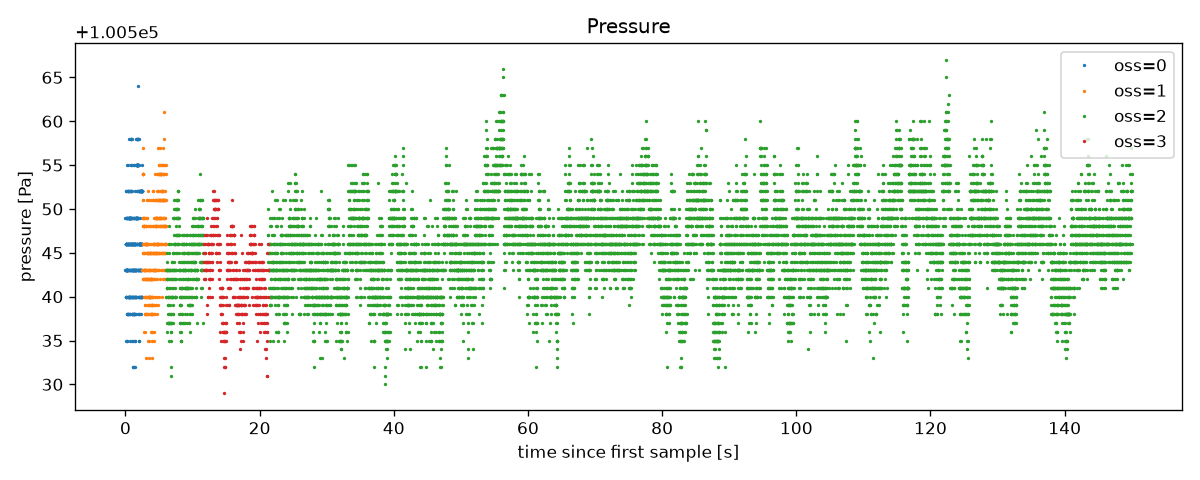
\includegraphics[width=\textwidth]{../E_analysis/figures/v2.0.0/pressure_series.png}
\end{center}

Fault behaviour was verified on earlier builds of the same sampler and is quoted
as such. Pulling SDA during a run, measured on the build immediately preceding
the current structure and recorded in \texttt{TESTING.md} section 10 (that
capture file is not among the committed ones), produced one \texttt{E 5}
(\texttt{EIO}) record 9\,995~$\mu$s after the last sample; samples stopped rather
than repeating with fresh timestamps, and the stream resumed on reconnect with no
reset, short by the outage divided by the cycle time (13\,088 samples against a
13\,663 baseline, zero drops).
Bus recovery was verified both ways on 1.5.0: forced on a healthy bus
(\texttt{20260830-131247}) it leaves the timing unchanged, and on a genuinely
wedged bus (\texttt{20260830-131424}, \texttt{-131457}) it recovers on the next
boot. The same failure on 1.4.0 killed three consecutive boots
(\texttt{20260830-131609} to \texttt{-131611}, zero samples) and required
reflashing to clear.

\subsection{Learning outcomes}

\todo[inline]{TO FILL IN: one bullet per member, in your own words. The
collective points below are true of the project and can stay; what is missing is
which of them each of you would put first, and what you expect to do with it.}

What the project taught us:

\begin{itemize}
\item \textbf{How a real-time kernel's device model fits together.} What it
  means for an IMFS node to \emph{own} a device, why the teardown order carries
  the safety argument, how an ioctl ABI is designed so it can be frozen, and how
  a bus driver and a device driver meet through a framework interface rather
  than through each other.
\item \textbf{That bringing up a peripheral means registers and nothing else.}
  Clock gating, alternate-function mux, CCR clock math; and that an I2C bus has
  a failure mode, a slave holding SDA low, that no amount of retrying fixes and
  that has to be designed for explicitly.
\item \textbf{That lock-free is a scheduling decision before it is a performance
  one.} The published snapshot is a seqlock because an RTEMS mutex held by a
  low-priority reader would block the acquisition task until the
  priority-inheritance handoff completed. The same reasoning sets the task
  priorities, and getting it wrong cost a measured 2.70~s console blackout.
\end{itemize}

We had no debugger on the running system, and print statements change the timing
they are supposed to observe, so the only way to know whether a change helped was
to emit raw records, capture them on the host and compute the statistics there.
Several of our defects were invisible in any single reading and obvious only in
the noise-versus-oversampling curve. The datasheet turned out to be a timing
contract as much as a feature list: the conversion-time table is a specification
the driver has to honour, and one tick of rounding against it was a real bug.

\paragraph{Questions that remained unanswered.} Self-heating at this duty cycle
is \emph{not} characterised: measured thermal drift varied by two orders of
magnitude between otherwise identical runs, and a much longer run is needed
before treating it as settled. One acceptance criterion, that RMS noise fall
monotonically at the OSS1 to OSS2 step, held in only one of five runs, and the
sweep design looks more likely at fault than the driver: the modes are visited
once each in sequence, so slow atmospheric drift lands on them unequally, and
the datasheet difference between those two modes is 1~Pa against run-to-run
scatter of about $\pm 1$~Pa. Interleaving the modes within a sweep is the change
we would make before trusting that criterion.

\paragraph{Tools we learned to use.} The RTEMS Source Builder and \texttt{waf}
for building a cross toolchain and a BSP; the \texttt{arm-rtems7} compiler,
\texttt{objcopy} and \texttt{objdump}; OpenOCD and the ST-Link for flashing and
for resetting the target from a script; \texttt{screen} and raw termios
programming for the serial console; \texttt{pandas} and \texttt{matplotlib} for
the host-side analysis; and Git branching and semantic versioning applied to
firmware, where a version number has to mean something about the measurement
path.

\subsection{Existing knowledge}

\todo[inline]{TO FILL IN: replace the list below with the courses you actually
took, and keep the one-line reason for each.}

\subsection{Problems encountered}
\label{sec:problems}

\begin{itemize}
\item \textbf{The BSP ships no I2C bus driver for the framework the device
  driver targets.} We found this only after the sensor driver was written: there
  was nothing for \texttt{i2c\_dev\_alloc\_and\_init()} to attach to. It roughly
  doubled the scope of the project; the 622-line polled STM32F4 master in
  \texttt{i2c/} exists because of it.

\item \textbf{Every \texttt{open()} returned \texttt{ENFILE}.} The RTEMS default
  for \texttt{CONFIGURE\_MAXIMUM\_FILE\_DESCRIPTORS} is 3, and
  \texttt{stdin}, \texttt{stdout} and \texttt{stderr} consume all three, so
  opening the bus node and the device node was impossible. The symptom (``too
  many open files'' on a system with two files) looked nothing like the cause.

\item \textbf{The console was silent for hours.} Two independent causes stacked:
  the stock BSP puts the console on USART3 while we had wired USART2, and on
  macOS the port must be opened as \texttt{/dev/cu.*} and never
  \texttt{/dev/tty.*}. A related trap cost another afternoon: termios settings
  applied with \texttt{stty -f} to a \texttt{cu.*} node are reset when the port
  is opened, so \texttt{cat} read at the driver's default baud and recorded
  framing garbage. The capture tool therefore applies them to an already-open
  descriptor and holds it for the whole run.

\item \textbf{A BSP header uses \texttt{or} as an identifier.} It compiles as C
  and cannot compile as C++, where \texttt{or} is an alternative spelling of
  \texttt{||}. Not a problem any of us had met before.

\item \textbf{Conversion waits expiring one tick early.}
  \texttt{rtems\_task\_wake\_after(n)} blocks for between $n-1$ and $n$ ticks,
  because the call lands somewhere inside the current tick. Our conversion
  timeouts used the datasheet maxima unpadded, so the driver occasionally read
  the result registers while the sensor was still converting, and still within
  specification. The defect was stochastic and invisible in any single reading;
  what exposed it was that RMS noise did not fall monotonically with
  oversampling, which it must. The fix is one tick of padding on every
  conversion constant, and the header says not to ``correct'' them back.

\item \textbf{The board came up dead after a reset, and stayed dead.} A CPU
  reset landing mid-transfer leaves the sensor holding SDA low; the peripheral
  latches BUSY and every transfer fails, across every subsequent reset. Only a
  power cycle cleared it. It reproduces in roughly two boots out of seven once
  bus occupancy is high, and the fix is the recovery sequence of Section
  \ref{sec:design}.

\item \textbf{A failing sampler starved the task that was supposed to report the
  failure.} On a successful cycle the sampler sleeps inside the conversion wait
  and yields; on a failing one the ioctl returns immediately, so a disconnected
  sensor turned it into a busy-loop at priority 2. Pulling SDA during a capture
  produced 2.70~s of complete console silence, no samples, no errors and no
  drops, because nothing below it could run. The sampler now yields a tick after
  a failed cycle, which is also the slot the consumer uses to notice and report
  the errno.

\item \textbf{A stale reading that looked fresh.} An early version stamped the
  last good measurement with the current timestamp when a cycle failed, so a
  dead sensor produced a plausible, perfectly-paced stream of a constant value,
  with nothing in the data to say anything was wrong. The layer now refuses to
  republish on a failed cycle, so the timestamp freezes and the age of the data
  stays visible. The header documents it, since the check cannot be forced on
  the consumer.

\item \textbf{Aliasing between the temperature cache and the noise
  statistics.} Compensation moves about 25~Pa per $0.1\,^{\circ}$C, so
  compensating a second of pressure readings against one cached temperature
  leaves the stream as a staircase: flat inside an interval, stepping when the
  cache refreshes. Whole-block RMS then measures thermal drift times the cache
  interval rather than sensor noise: 16.21~Pa against 4.85~Pa within-segment in
  one measured block. The analysis now splits each block at the cache refreshes
  and reports the median within-segment RMS.

\item \textbf{A use-after-free in teardown.} Freeing the device directly leaves
  a published IMFS node pointing at freed memory. The correct order is
  \texttt{unlink()}, which runs the node's destroy handler. Nothing in a normal
  run ever tears the device down, so the whole path was dead code, which is
  where the bug lived; it is now exercised under a build flag that registers,
  opens, unlinks and re-opens once at boot.
\end{itemize}

\section{Honor Pledge}
(\textbf{This part cannot be modified and it is mandatory to sign it})

I/We pledge that this work was fully and wholly completed within the criteria
established for academic integrity by Politecnico di Milano (Code of Ethics and
Conduct) and represents my/our original production, unless otherwise cited.

I/We also understand that this project, if successfully graded,  will fulfill part B requirement of the
Advanced Operating System course and that it will be considered valid up until
the AOS exam of Sept. 2022. 

\begin{flushright}
Group Students' signatures
\end{flushright}


\end{document}
